\documentclass[
    language=english,
    doctype=zine,
    institution=none,
]{../../omnilatex}

\RequirePackage{config/document-settings}

\begin{document}
\maketitle

\vspace{0.5cm}

\begin{center}
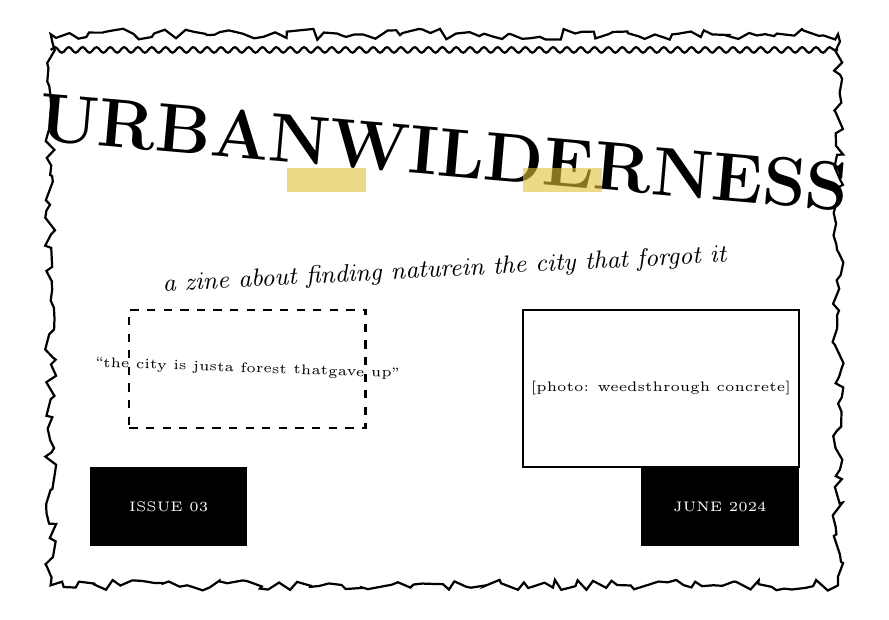
\begin{tikzpicture}
    % Zine cover - rough, cut-and-paste aesthetic
    \draw[thick, decorate, decoration={random steps, segment length=3pt, amplitude=2pt}] (0,0) rectangle (10,7);
    
    % Title - hand-drawn style
    \node[font=\fontsize{36}{40}\selectfont\bfseries, rotate=-5] at (5,5.5) {URBAN\\WILDERNESS};
    
    % Subtitle
    \node[font=\small\itshape, rotate=3] at (5,4) {a zine about finding nature\\in the city that forgot it};
    
    % Cut-out letters style
    \fill[black] (0.5,0.5) rectangle (2.5,1.5);
    \node[white, font=\tiny] at (1.5,1) {ISSUE 03};
    \fill[black] (7.5,0.5) rectangle (9.5,1.5);
    \node[white, font=\tiny] at (8.5,1) {JUNE 2024};
    
    % Collage elements
    \draw[thick, dashed] (1,2) -- (4,2) -- (4,3.5) -- (1,3.5) -- cycle;
    \node[font=\tiny, rotate=-2] at (2.5,2.75) { ``the city is just\\a forest that\\gave up''};
    
    % Tape strips
    \fill[yellow!50!brown, opacity=0.6] (3,5) rectangle (4,5.3);
    \fill[yellow!50!brown, opacity=0.6] (6,5) rectangle (7,5.3);
    
    % Photo placeholder
    \draw[thick] (6,1.5) rectangle (9.5,3.5);
    \node[font=\tiny] at (7.75,2.5) {[photo: weeds\\through concrete]};
    
    % Hand-drawn border
    \draw[thick, decorate, decoration={snake, amplitude=1pt, segment length=5pt}] (0,6.8) -- (10,6.8);
\end{tikzpicture}
\end{center}

\vspace{0.5cm}

\begin{center}
\textit{``Every crack in the sidewalk is an invitation.''}
\end{center}

\vspace{0.5cm}

\section*{EDITOR'S NOTE}

Hey there,

This is issue three of \textit{Urban Wilderness}, and I'm writing this at 2 AM in a laundromat on Atlantic Avenue because my apartment doesn't have Wi-Fi and the coffee shop down the street closed an hour ago. The dryer is making a sound like a dying animal, and there's a cat sleeping on top of the folding table who I'm pretty sure doesn't live here.

I started this zine because I got tired of people telling me cities are ugly. They're not. They're just different kinds of beautiful. You have to look closer. You have to pay attention to the things that grow in the spaces we've forgotten---the dandelions pushing through asphalt, the moss on the north side of buildings, the pigeons that have figured out how to use crosswalk signals.

This issue is about weeds. Not the kind you pull out of your garden---the kind that pull themselves out of concrete. The kind that refuse to go away. The kind that remind us that nature doesn't care about our sidewalks and our parking lots and our carefully planned urban landscapes. Nature just grows.

Anyway. The dryer just stopped, so I have to go fold my clothes before someone takes my machine. Enjoy the zine. Leave a copy somewhere unexpected when you're done with it.

--- J.

\vspace{0.5cm}

\section*{THE FIELD GUIDE TO URBAN WEEDS}

\begin{center}
\begin{minipage}{0.9\textwidth}

\textbf{DANDELION} (\textit{Taraxacum officinale})

The classic. The rebel. The weed that launched a thousand childhood wishes. Dandelions are the first sign that nature hasn't given up on your neighborhood. They grow in sidewalk cracks, parking lot medians, and the neglected strips of earth between buildings that nobody claims.

Fun fact: Every part of a dandelion is edible. The leaves make a bitter salad. The flowers can be fried into fritters. The roots can be roasted into a coffee substitute that tastes vaguely of disappointment but is technically nutritious.

Where to find them: Everywhere. Seriously. Look down.

\vspace{0.3cm}

\textbf{PURSLANE} (\textit{Portulaca oleracea})

Purslane is the succulent of the weed world. It has thick, fleshy leaves and a taste like lemon pepper. It grows low to the ground, spreading out in a starburst pattern that looks like it's trying to hug the concrete.

In some cultures, purslane is a delicacy. In your neighborhood, it's probably growing in the crack next to your front door, and you've been stepping on it every day without realizing it's one of the most nutritious greens on the planet.

Where to find it: Sunny spots with poor soil. Parking lot edges. The base of chain-link fences.

\vspace{0.3cm}

\textbf{LAMB'S QUARTERS} (\textit{Chenopodium album})

Lamb's quarters look like tiny, dusty versions of spinach, which makes sense because they're in the same family. They grow tall and bushy, often reaching three or four feet in abandoned lots and along railroad tracks.

The leaves are covered in a white, powdery coating that looks like someone dusted them with flour. This is not a defect. This is nature's sunscreen. Lamb's quarters are edible, nutritious, and probably growing in that vacant lot you walk past every day.

Where to find it: Disturbed soil. Construction sites. Anywhere humans have dug up the earth and then walked away.

\vspace{0.3cm}

\textbf{PLANTAIN} (\textit{Plantago major})

Not the banana kind. The ``oh, that thing in my yard'' kind. Plantain is a broad-leafed weed with leaves that look like they were designed by a government committee---functional, symmetrical, and completely uninteresting.

Except that plantain has been used as medicine for thousands of years. The leaves can be chewed and applied to insect bites to reduce swelling. The seeds are a natural laxative. The whole plant is edible, though I wouldn't recommend it unless you're really committed to the ``eating weeds'' lifestyle.

Where to find it: Lawns, sidewalks, and the edges of parking lots. It thrives in compacted soil, which is why it loves urban environments so much.

\vspace{0.3cm}

\textbf{MOTHERWORT} (\textit{Leonurus cardiaca})

Motherwort is a medicinal herb that escaped from someone's garden sometime in the 1800s and has been living wild ever since. It grows tall---six feet or more---with spiky, trumpet-shaped flowers that bees love and humans mostly ignore.

The name ``motherwort'' comes from its traditional use as a remedy for women's health issues. It's also been used for anxiety, insomnia, and heart palpitations. Modern science is divided on whether it actually works, but the bees don't care about modern science, and neither should you.

Where to find it: Along fences, behind abandoned buildings, and in the kind of overgrown lots where you expect to find raccoons having a meeting.

\end{minipage}
\end{center}

\section*{PHOTO ESSAY: WEEDS OF ATLANTIC AVENUE}

\begin{center}
\begin{minipage}{0.9\textwidth}

\textbf{Plate 1:} Dandelion growing through a crack in the sidewalk outside the bodega on the corner. The crack is maybe half an inch wide. The dandelion doesn't care. It has rooted itself in the thin layer of dirt that accumulates in sidewalk cracks over years, and it is thriving. There are three blooms, two of which have already gone to seed. A passing pedestrian has stepped on one of the seed heads, scattering the next generation across the concrete.

\textbf{Plate 2:} Purslane colonizing the base of a parking meter on the north side of the street. The parking meter is broken. The purslane is not. The leaves are thick and green, radiating outward from a central stem in a pattern that looks like a green explosion frozen in time. Someone has stuck a cigarette butt in the soil next to it. The purslane is unbothered.

\textbf{Plate 3:} A row of lamb's quarters growing along the base of a chain-link fence surrounding a vacant lot. The lot is full of construction debris---broken concrete, twisted rebar, plastic bags tangled in weeds. But the lamb's quarters have found a strip of exposed earth along the fence line, and they've claimed it. They stand three feet tall, their dusty leaves catching the afternoon light.

\textbf{Plate 4:} Motherwort growing behind an abandoned warehouse on the south side of the avenue. The warehouse has been empty for at least a decade. The motherwort has been growing here for at least that long, spreading outward from the original plant into a small grove. The flowers are in bloom, purple and white, and the bees are everywhere, drunk on nectar, stumbling from flower to flower like patrons at a bar at closing time.

\textbf{Plate 5:} A single plantain leaf growing through a crack in a manhole cover. The manhole cover is cast iron, solid, immovable. The plantain doesn't care. It has found the one imperfection in the metal, the one spot where the crack runs deep enough to reach the soil below, and it has pushed a leaf through. The leaf is broad and green and utterly indifferent to the fact that it is growing through a hole designed to withstand the weight of city buses.

\end{minipage}
\end{center}

\section*{DIY: MAKING WEED TEA}

What you'll need:
\begin{itemize}
    \item A handful of dandelion leaves (washed)
    \item A handful of lamb's quarters (washed)
    \item Two cups of boiling water
    \item Honey or lemon (optional, recommended)
    \item A sense of adventure
    \item A willingness to admit that you're drinking weeds and that this is somehow fine
\end{itemize}

Steps:
\begin{enumerate}
    \item Put the leaves in a mug. Don't be precious about it. Just stuff them in there.
    \item Pour the boiling water over the leaves. Let it steep for ten minutes. The water will turn green. This is normal. This is good.
    \item Strain the leaves. Add honey or lemon if you want to pretend this is a normal beverage.
    \item Drink. Reflect on the fact that you just made tea from plants that most people spray with poison.
    \item Consider that maybe---just maybe---the weeds have been trying to feed us all along, and we've been too busy building parking lots to notice.
\end{enumerate}

\section*{THE WEED MANIFESTO}

\begin{enumerate}
    \item A weed is a plant that has chosen to grow where we didn't ask it to.
    \item A weed is not a failure of gardening. It is a success of biology.
    \item Weeds don't need our permission. They don't need our approval. They don't need our water, our fertilizer, or our carefully curated garden beds.
    \item Weeds grow in cracks. Weeds grow in rubble. Weeds grow in the places we've abandoned and the spaces we've forgotten.
    \item Weeds are not ugly. They are just different kinds of beautiful.
    \item Weeds are resilient. Weeds are persistent. Weeds are, in their own quiet way, magnificent.
    \item If you can't find beauty in a dandelion growing through a sidewalk, the problem is not the dandelion.
    \item Weeds are the city's way of reminding us that nature doesn't care about our plans.
    \item And honestly? That's kind of comforting.
\end{enumerate}

\vspace{0.5cm}

\begin{center}
\textit{``The earth is not given to you by your parents.\\
It is lent to you by your children.''}\\
--- Native American proverb
\end{center}

\vspace{0.5cm}

\section*{CONTRIBUTIONS}

\textit{Urban Wilderness} accepts submissions of writing, photography, art, and random thoughts about nature in the city. Send your stuff to:

\begin{quote}
Urban Wilderness Zine\\
c/o J. Hartwell\\
42 Atlantic Avenue, Apt. 3B\\
Brooklyn, NY 11201
\end{quote}

Or just leave a copy of your work somewhere we'll find it. We're good at noticing things growing in unexpected places.

\vspace{0.5cm}

\begin{center}
\textbf{ISSUE 03 --- JUNE 2024 --- PRINT RUN: 200}\\
\textit{Made with love, a stapler, and too much coffee.}
\end{center}

\end{document}
